\begin{figure}[H]
    \centering
    \scriptsize
    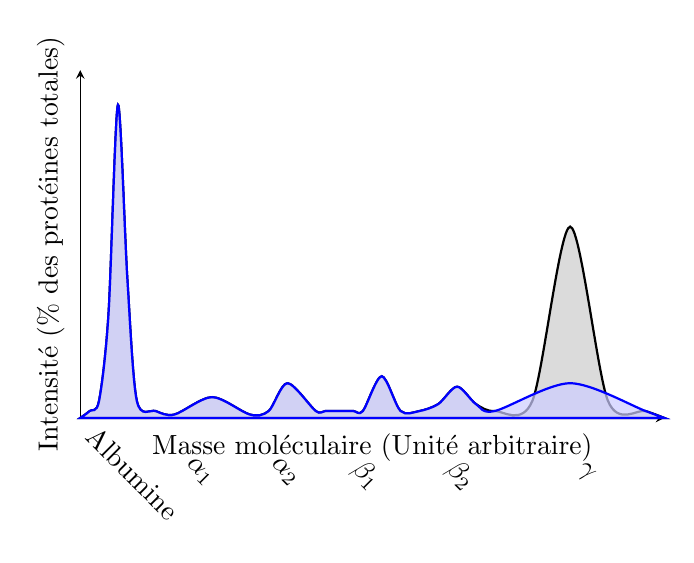
\begin{tikzpicture}
        \begin{axis}[
            width=9cm,
            height=6cm,
            xlabel={Masse moléculaire (Unité arbitraire)},
            ylabel={Intensité (\% des protéines totales)},
            ymin=0, ymax=100,
            axis y line=left,
            axis x line=bottom,
            ytick=\empty,
            xtick=\empty,
            clip=false,
            grid=none,
            enlarge x limits=false
        ]   

        % Profil avec pic monoclonal
        \addplot[
            thick, black, smooth,
            fill=black!20, fill opacity=0.7
        ] coordinates {
            (0, 0)
            (0.5, 2) 
            (1, 5) 
            (1.5, 30) 
            (2, 90) 
            (2.5, 40) 
            (3, 5) 
            (4, 2) 
            (5, 1)  
            (7, 6)
            (9, 1)  
            (10, 2) 
            (11, 10) 
            (12.5, 2) 
            (13, 2)
            (14, 2)  
            (14.5, 2)
            (15, 2) 
            (16, 12) 
            (17, 2) 
            (18, 2)  
            (19, 4) 
            (20, 9) 
            (21, 4) 
            (22, 2) 
            (24, 5) 
            (26, 55) 
            (28, 5) 
            (30, 2) 
            (31, 0)   
        } -- cycle;

        % Profil normal
        \addplot[
            thick, blue, smooth,
            fill=blue!20, fill opacity=0.7
        ] coordinates {
            (0, 0)
            (0.5, 2) 
            (1, 5) 
            (1.5, 30) 
            (2, 90) 
            (2.5, 40) 
            (3, 5) 
            (4, 2) 
            (5, 1)  
            (7, 6)
            (9, 1)  
            (10, 2) 
            (11, 10) 
            (12.5, 2) 
            (13, 2)
            (14, 2)  
            (14.5, 2)
            (15, 2) 
            (16, 12) 
            (17, 2) 
            (18, 2)  
            (19, 4) 
            (20, 9) 
            (21, 4) 
            (22, 2)  
            (26, 10) 
            (30, 2) 
            (31, 0)            
        } -- cycle;

        \node[rotate=-45, anchor=north] at (axis cs:3.5, -12) {Albumine};
        \node[rotate=-45, anchor=north] at (axis cs:7, -12) {$\alpha_1$};
        \node[rotate=-45, anchor=north] at (axis cs:11.5, -12) {$\alpha_2$};
        \node[rotate=-45, anchor=north] at (axis cs:16, -12) {$\beta_1$};
        \node[rotate=-45, anchor=north] at (axis cs:21, -12) {$\beta_2$};
        \node[rotate=-45, anchor=north] at (axis cs:27.5, -12) {$\gamma$};

        \end{axis}
    \end{tikzpicture}
\end{figure}
